% Options for packages loaded elsewhere
% Options for packages loaded elsewhere
\PassOptionsToPackage{unicode}{hyperref}
\PassOptionsToPackage{hyphens}{url}
%
\documentclass[
  ignorenonframetext,
  aspectratio=169,
  russian,
]{beamer}
\newif\ifbibliography
\usepackage{pgfpages}
\setbeamertemplate{caption}[numbered]
\setbeamertemplate{caption label separator}{: }
\setbeamercolor{caption name}{fg=normal text.fg}
\beamertemplatenavigationsymbolshorizontal
% remove section numbering
\setbeamertemplate{part page}{
  \centering
  \begin{beamercolorbox}[sep=16pt,center]{part title}
    \usebeamerfont{part title}\insertpart\par
  \end{beamercolorbox}
}
\setbeamertemplate{section page}{
  \centering
  \begin{beamercolorbox}[sep=12pt,center]{section title}
    \usebeamerfont{section title}\insertsection\par
  \end{beamercolorbox}
}
\setbeamertemplate{subsection page}{
  \centering
  \begin{beamercolorbox}[sep=8pt,center]{subsection title}
    \usebeamerfont{subsection title}\insertsubsection\par
  \end{beamercolorbox}
}
% Prevent slide breaks in the middle of a paragraph
\widowpenalties 1 10000
\raggedbottom
\AtBeginPart{
  \frame{\partpage}
}
\AtBeginSection{
  \ifbibliography
  \else
    \frame{\sectionpage}
  \fi
}
\AtBeginSubsection{
  \frame{\subsectionpage}
}
\usepackage{iftex}
\ifPDFTeX
  \usepackage[T1]{fontenc}
  \usepackage[utf8]{inputenc}
  \usepackage{textcomp} % provide euro and other symbols
\else % if luatex or xetex
  \usepackage{unicode-math} % this also loads fontspec
  \defaultfontfeatures{Scale=MatchLowercase}
  \defaultfontfeatures[\rmfamily]{Ligatures=TeX,Scale=1}
\fi
\usepackage{lmodern}

\usetheme[]{metropolis}
\ifPDFTeX\else
  % xetex/luatex font selection
\fi
% Use upquote if available, for straight quotes in verbatim environments
\IfFileExists{upquote.sty}{\usepackage{upquote}}{}
\IfFileExists{microtype.sty}{% use microtype if available
  \usepackage[]{microtype}
  \UseMicrotypeSet[protrusion]{basicmath} % disable protrusion for tt fonts
}{}


\usepackage{longtable,booktabs,array}
\usepackage{calc} % for calculating minipage widths
\usepackage{caption}
% Make caption package work with longtable
\makeatletter
\def\fnum@table{\tablename~\thetable}
\makeatother
\usepackage{graphicx}
\makeatletter
\newsavebox\pandoc@box
\newcommand*\pandocbounded[1]{% scales image to fit in text height/width
  \sbox\pandoc@box{#1}%
  \Gscale@div\@tempa{\textheight}{\dimexpr\ht\pandoc@box+\dp\pandoc@box\relax}%
  \Gscale@div\@tempb{\linewidth}{\wd\pandoc@box}%
  \ifdim\@tempb\p@<\@tempa\p@\let\@tempa\@tempb\fi% select the smaller of both
  \ifdim\@tempa\p@<\p@\scalebox{\@tempa}{\usebox\pandoc@box}%
  \else\usebox{\pandoc@box}%
  \fi%
}
% Set default figure placement to htbp
\def\fps@figure{htbp}
\makeatother



\ifLuaTeX
\usepackage[bidi=basic,provide=*]{babel}
\else
\usepackage[bidi=default,provide=*]{babel}
\fi
% get rid of language-specific shorthands (see #6817):
\let\LanguageShortHands\languageshorthands
\def\languageshorthands#1{}


\setlength{\emergencystretch}{3em} % prevent overfull lines

\providecommand{\tightlist}{%
  \setlength{\itemsep}{0pt}\setlength{\parskip}{0pt}}



 

\usepackage[]{csquotes}

\IfFileExists{plex-otf.sty}{
  %% Full TeXlive
  % \usepackage[%
  %   % math,
  %   RM={Scale=0.94},SS={Scale=0.94},SScon={Scale=0.94},TT={Scale=MatchLowercase,FakeStretch=0.9},DefaultFeatures={Ligatures=Common}
  % ]{plex-otf}
}{
  %% TinyTeX
  \usepackage{libertine}
}

%%% Load theme
% https://deic.uab.cat/~iblanes/beamer_gallery/
\IfFileExists{beamerthemegotham.sty}{
  %% Full TeXlive
  \usetheme{gotham}
  \gothamset{
    numbering=totalpagenumber,
    parttocframe default=off,
    sectiontocframe default=off,
    subsectiontocframe default=off,
  }
}{
  %% TinyTeX
  \usetheme{Madrid}
}
\metroset{progressbar=frametitle,sectionpage=progressbar,numbering=fraction}
\makeatletter
\beamer@ignorenonframefalse
\makeatother
\makeatletter
\@ifpackageloaded{caption}{}{\usepackage{caption}}
\AtBeginDocument{%
\ifdefined\contentsname
  \renewcommand*\contentsname{Содержание}
\else
  \newcommand\contentsname{Содержание}
\fi
\ifdefined\listfigurename
  \renewcommand*\listfigurename{Список иллюстраций}
\else
  \newcommand\listfigurename{Список иллюстраций}
\fi
\ifdefined\listtablename
  \renewcommand*\listtablename{Список таблиц}
\else
  \newcommand\listtablename{Список таблиц}
\fi
\ifdefined\figurename
  \renewcommand*\figurename{Рисунок}
\else
  \newcommand\figurename{Рисунок}
\fi
\ifdefined\tablename
  \renewcommand*\tablename{Таблица}
\else
  \newcommand\tablename{Таблица}
\fi
}
\@ifpackageloaded{float}{}{\usepackage{float}}
\floatstyle{ruled}
\@ifundefined{c@chapter}{\newfloat{codelisting}{h}{lop}}{\newfloat{codelisting}{h}{lop}[chapter]}
\floatname{codelisting}{Список}
\newcommand*\listoflistings{\listof{codelisting}{Листинги}}
\makeatother
\makeatletter
\makeatother
\makeatletter
\@ifpackageloaded{caption}{}{\usepackage{caption}}
\@ifpackageloaded{subcaption}{}{\usepackage{subcaption}}
\makeatother

\usepackage{bookmark}
\IfFileExists{xurl.sty}{\usepackage{xurl}}{} % add URL line breaks if available
\urlstyle{same}
\hypersetup{
  pdftitle={Лабораторная работа 3},
  pdfauthor={Самарханова Полина Тимуровна.},
  pdflang={ru-RU},
  hidelinks,
  pdfcreator={LaTeX via pandoc}}


\title{Лабораторная работа 3}
\subtitle{иммитационное моделирование}
\author{Самарханова Полина Тимуровна.}
\date{Invalid Date}
\institute{Российский университет дружбы народов, Москва, Россия}

\begin{document}
\frame{\titlepage}


\begin{frame}{Задания}
\phantomsection\label{ux437ux430ux434ux430ux43dux438ux44f}
\begin{itemize}[<+->]
\tightlist
\item
  Создать рабочий каталог для всего курса. -Установить необходимые
  пакеты.
\item
  Выполнить предложенный код.
\item
  Преобразовать код в литературный стиль.
\item
  Сгенерировать из литературного кода:

  \begin{itemize}[<+->]
  \tightlist
  \item
    чистый код;
  \item
    jupyter notebook;
  \item
    документацию в формате Quarto.
  \end{itemize}
\item
  Выполнить код из jupyter notebook.
\item
  Интегрировать документацию в формате Quarto в отчёт.
\item
  Добавить в код в литературном стиле вычисление для набора параметров.
\item
  Сгенерировать из литературного кода с параметрами:

  \begin{itemize}[<+->]
  \tightlist
  \item
    чистый код;
  \item
    jupyter notebook;
  \item
    документацию в формате Quarto.
  \end{itemize}
\item
  Выполнить код из jupyter notebook с параметрами.
\item
  Интегрировать документацию с параметрами в формате Quarto в отчёт.
\end{itemize}
\end{frame}

\begin{frame}{Цели и задачи}
\phantomsection\label{ux446ux435ux43bux438-ux438-ux437ux430ux434ux430ux447ux438}
\begin{itemize}[<+->]
\tightlist
\item
  Целью данной лабораторной работы является освоение методологии
  агентного моделирования (Agent-Based Modeling, ABM) на примере модели
  Daisyworld, а также приобретение практических навыков разработки,
  визуализации и анализа агентных моделей с использованием пакета
  Agents.jl в среде Julia.
\end{itemize}
\end{frame}

\section{Выполнение}\label{ux432ux44bux43fux43eux43bux43dux435ux43dux438ux435}

\begin{frame}{Реализация на Agents.jl}
\phantomsection\label{ux440ux435ux430ux43bux438ux437ux430ux446ux438ux44f-ux43dux430-agents.jl}
Перехожу в каталог лабораторной работы 3 и создаю папку scr и файл
daisyworld.jl

\begin{figure}[H]

{\centering \pandocbounded{
\includegraphics[keepaspectratio]{image/1.png}}

}

\caption{создание файла}

\end{figure}%
\end{frame}

\begin{frame}{}
\phantomsection\label{section}
В открывшемся окне вставила код из методички

\begin{figure}[H]

{\centering \pandocbounded{
\includegraphics[keepaspectratio]{image/2.png}}

}

\caption{Тектовый редактор}

\end{figure}%
\end{frame}

\begin{frame}{}
\phantomsection\label{section-1}
Установила необходимые пакеты

\begin{figure}[H]

{\centering \pandocbounded{
\includegraphics[keepaspectratio]{image/3.png}}

}

\caption{установка пакетов}

\end{figure}%
\end{frame}

\begin{frame}{}
\phantomsection\label{section-2}
Подключила файл с моделью

\begin{figure}[H]

{\centering \pandocbounded{
\includegraphics[keepaspectratio]{image/4.png}}

}

\caption{подключение}

\end{figure}%
\end{frame}

\begin{frame}{}
\phantomsection\label{section-3}
Создала модель

\begin{figure}[H]

{\centering \pandocbounded{
\includegraphics[keepaspectratio]{image/5.png}}

}

\caption{модель}

\end{figure}%
\end{frame}

\begin{frame}{}
\phantomsection\label{section-4}
Запустила программу и получил результат

\begin{figure}[H]

{\centering \pandocbounded{
\includegraphics[keepaspectratio]{image/6.png}}

}

\caption{результат}

\end{figure}%
\end{frame}

\begin{frame}{Базовая визуализация}
\phantomsection\label{ux431ux430ux437ux43eux432ux430ux44f-ux432ux438ux437ux443ux430ux43bux438ux437ux430ux446ux438ux44f}
Установила необходимые пакеты

\begin{figure}[H]

{\centering \pandocbounded{
\includegraphics[keepaspectratio]{image/7.png}}

}

\caption{установка пакетов}

\end{figure}%
\end{frame}

\begin{frame}{}
\phantomsection\label{section-5}
Создала файл scripts/daisyworld.jl

\begin{figure}[H]

{\centering \pandocbounded{
\includegraphics[keepaspectratio]{image/8.png}}

}

\caption{файл}

\end{figure}%
\end{frame}

\begin{frame}{}
\phantomsection\label{section-6}
В открывшемся окне вставила код из медодички

\begin{figure}[H]

{\centering \pandocbounded{
\includegraphics[keepaspectratio]{image/9.png}}

}

\caption{код}

\end{figure}%
\end{frame}

\begin{frame}{}
\phantomsection\label{section-7}
Запустила код

\begin{figure}[H]

{\centering \pandocbounded{
\includegraphics[keepaspectratio]{image/10.png}}

}

\caption{запуск}

\end{figure}%
\end{frame}

\begin{frame}{}
\phantomsection\label{section-8}
Посмотрела результат

\begin{figure}[H]

{\centering \pandocbounded{
\includegraphics[keepaspectratio]{image/11.png}}

}

\caption{графики}

\end{figure}%
\end{frame}

\begin{frame}{}
\phantomsection\label{section-9}
Открыла файл для литературного кода

\begin{figure}[H]

{\centering \pandocbounded{
\includegraphics[keepaspectratio]{image/14.png}}

}

\caption{файл}

\end{figure}%
\end{frame}

\begin{frame}{}
\phantomsection\label{section-10}
В открывшеся окне вставила литературный код

\begin{figure}[H]

{\centering \pandocbounded{
\includegraphics[keepaspectratio]{image/15.png}}

}

\caption{запуск LV}

\end{figure}%
\end{frame}

\begin{frame}{}
\phantomsection\label{section-11}
Сгенерировала чистый код

\begin{figure}[H]

{\centering \pandocbounded{
\includegraphics[keepaspectratio]{image/16.png}}

}

\caption{генерируем чистый код}

\end{figure}%
\end{frame}

\begin{frame}{}
\phantomsection\label{section-12}
Запустила код из юпитера

\begin{figure}[H]

{\centering \pandocbounded{
\includegraphics[keepaspectratio]{image/17.png}}

}

\caption{запуск кода из юпитера}

\end{figure}%
\end{frame}

\begin{frame}{Анимация модели}
\phantomsection\label{ux430ux43dux438ux43cux430ux446ux438ux44f-ux43cux43eux434ux435ux43bux438}
Установила необходимые пакеты

\begin{figure}[H]

{\centering \pandocbounded{
\includegraphics[keepaspectratio]{image/19.png}}

}

\caption{файл}

\end{figure}%
\end{frame}

\begin{frame}{}
\phantomsection\label{section-13}
В открывшемся окне вставила код из медодички

\begin{figure}[H]

{\centering \pandocbounded{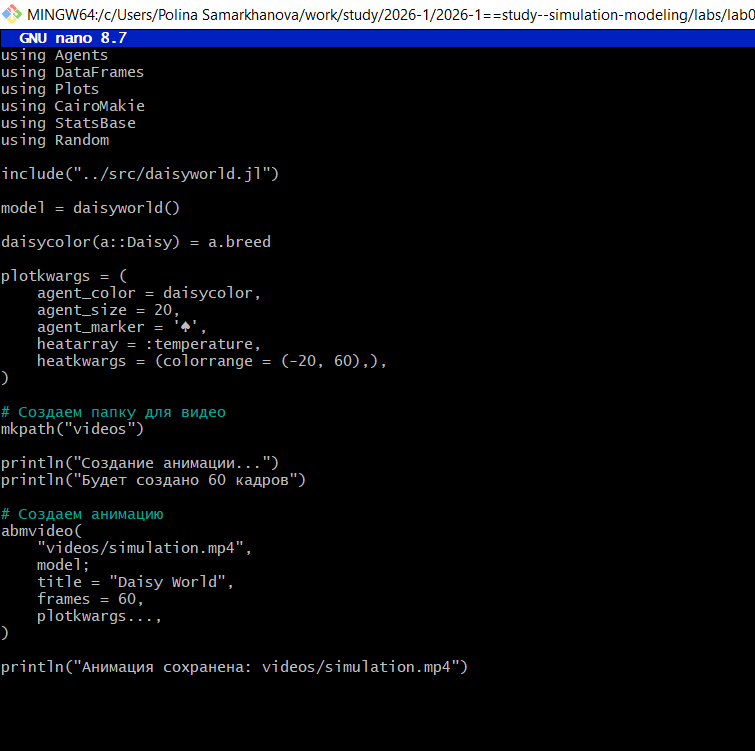
\includegraphics[keepaspectratio]{image/20.png}}

}

\caption{код}

\end{figure}%
\end{frame}

\begin{frame}{}
\phantomsection\label{section-14}
Запустила код, видео выложила на платформы

\begin{figure}[H]

{\centering \pandocbounded{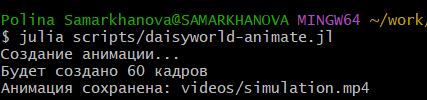
\includegraphics[keepaspectratio]{image/21.png}}

}

\caption{запуск}

\end{figure}%
\end{frame}

\begin{frame}{Динамика числа маргариток}
\phantomsection\label{ux434ux438ux43dux430ux43cux438ux43aux430-ux447ux438ux441ux43bux430-ux43cux430ux440ux433ux430ux440ux438ux442ux43eux43a}
Создала файл scripts/daisyworld-count.jl

\begin{figure}[H]

{\centering \pandocbounded{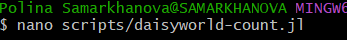
\includegraphics[keepaspectratio]{image/22.png}}

}

\caption{файл}

\end{figure}%
\end{frame}

\begin{frame}{}
\phantomsection\label{section-15}
В открывшемся окне вставила код из медодички

\begin{figure}[H]

{\centering \pandocbounded{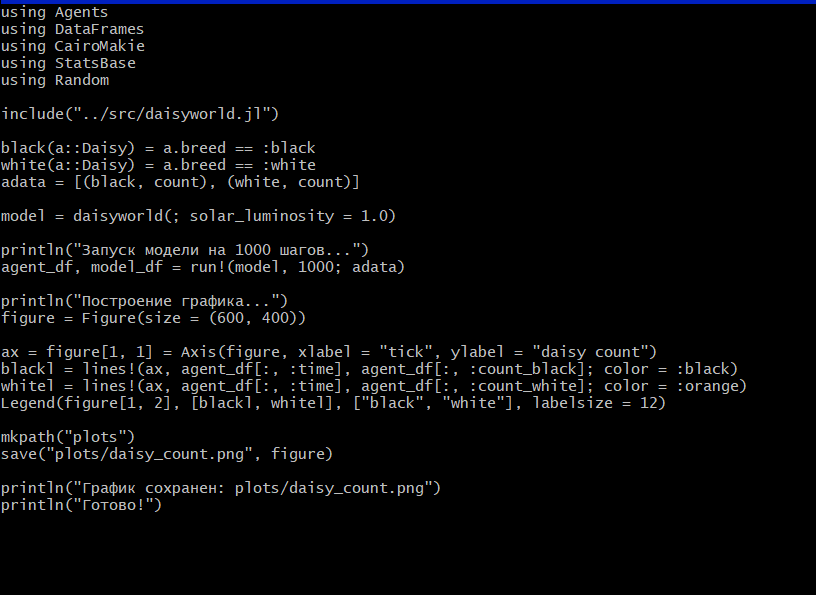
\includegraphics[keepaspectratio]{image/23.png}}

}

\caption{код}

\end{figure}%
\end{frame}

\begin{frame}{}
\phantomsection\label{section-16}
Запустила код

\begin{figure}[H]

{\centering \pandocbounded{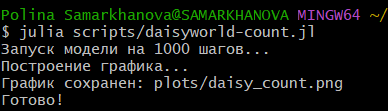
\includegraphics[keepaspectratio]{image/24.png}}

}

\caption{запуск}

\end{figure}%
\end{frame}

\begin{frame}{}
\phantomsection\label{section-17}
Посмотрела результат

\begin{figure}[H]

{\centering \pandocbounded{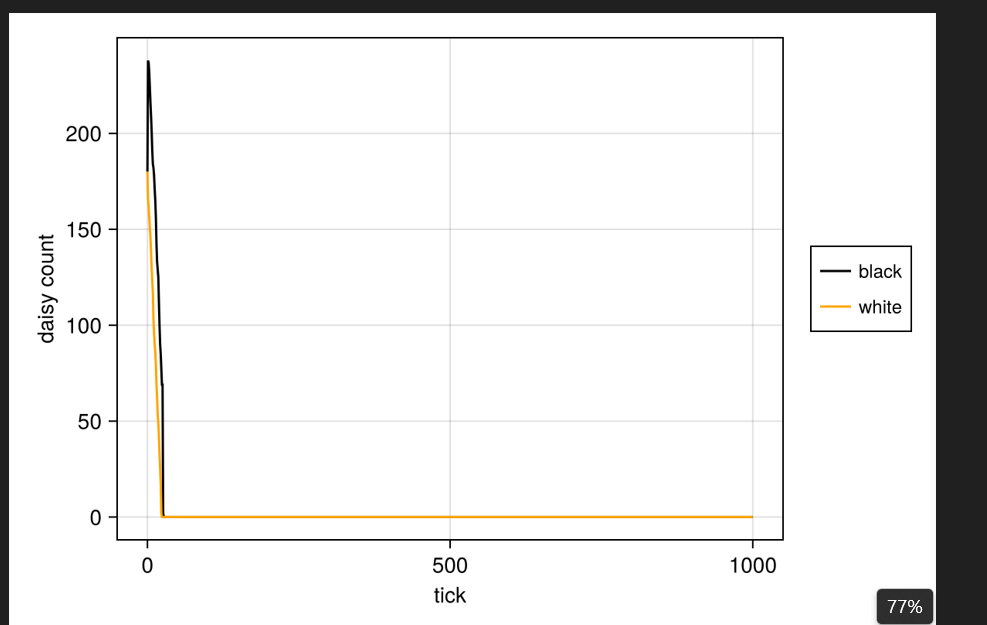
\includegraphics[keepaspectratio]{image/25.png}}

}

\caption{графики}

\end{figure}%
\end{frame}

\begin{frame}{Динамика модели}
\phantomsection\label{ux434ux438ux43dux430ux43cux438ux43aux430-ux43cux43eux434ux435ux43bux438}
Создала файл scripts/daisyworld-luminosity.jl

\begin{figure}[H]

{\centering \pandocbounded{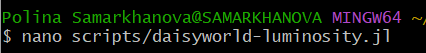
\includegraphics[keepaspectratio]{image/26.png}}

}

\caption{файл}

\end{figure}%
\end{frame}

\begin{frame}{}
\phantomsection\label{section-18}
В открывшемся окне вставила код из медодички

\begin{figure}[H]

{\centering \pandocbounded{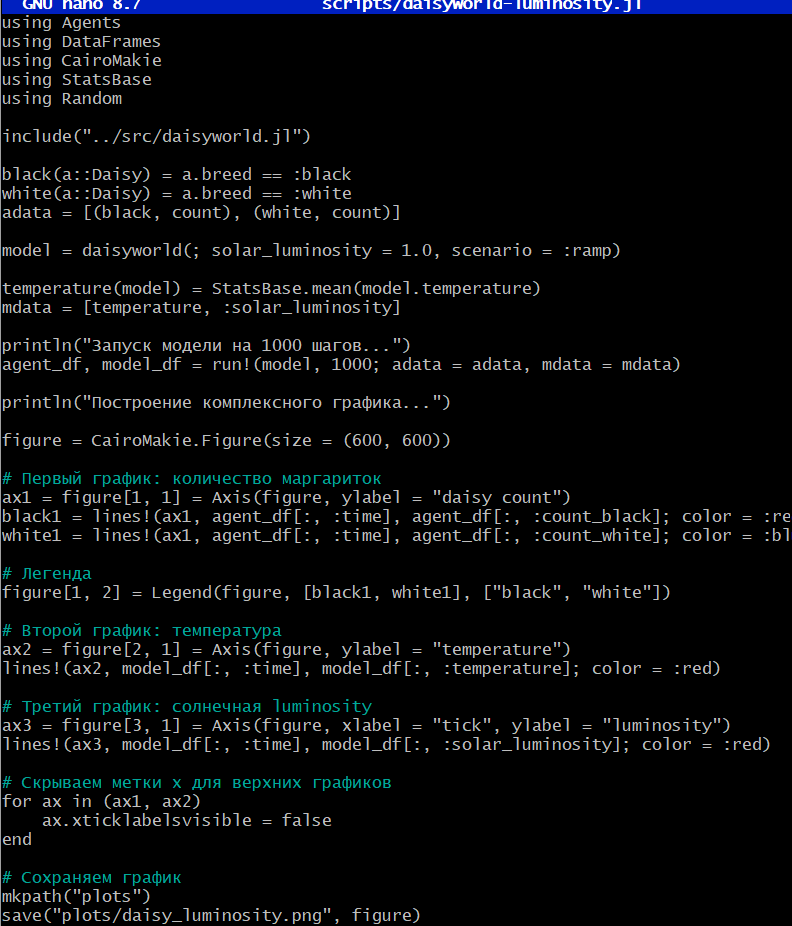
\includegraphics[keepaspectratio]{image/27.png}}

}

\caption{код}

\end{figure}%
\end{frame}

\begin{frame}{}
\phantomsection\label{section-19}
Запустила код

\begin{figure}[H]

{\centering \pandocbounded{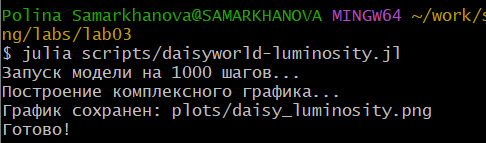
\includegraphics[keepaspectratio]{image/28.png}}

}

\caption{запуск}

\end{figure}%
\end{frame}

\begin{frame}{}
\phantomsection\label{section-20}
Посмотрела результат

\begin{figure}[H]

{\centering \pandocbounded{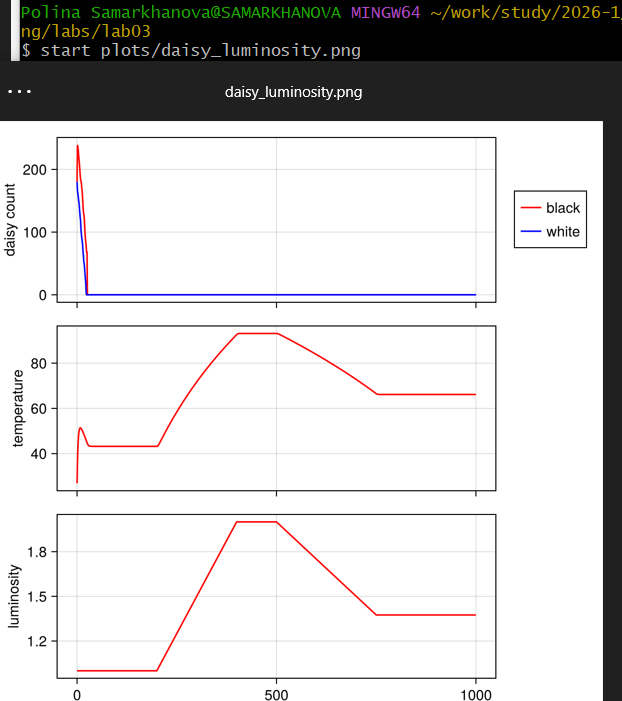
\includegraphics[keepaspectratio]{image/29.png}}

}

\caption{графики}

\end{figure}%
\end{frame}

\begin{frame}{Базовая визуализация(параметры)}
\phantomsection\label{ux431ux430ux437ux43eux432ux430ux44f-ux432ux438ux437ux443ux430ux43bux438ux437ux430ux446ux438ux44fux43fux430ux440ux430ux43cux435ux442ux440ux44b}
Создала файл scripts/daisyworld\_param.jl

\begin{figure}[H]

{\centering \pandocbounded{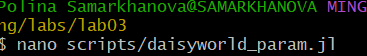
\includegraphics[keepaspectratio]{image/30.png}}

}

\caption{файл}

\end{figure}%
\end{frame}

\begin{frame}{}
\phantomsection\label{section-21}
В открывшемся окне вставила код из медодички

\begin{figure}[H]

{\centering \pandocbounded{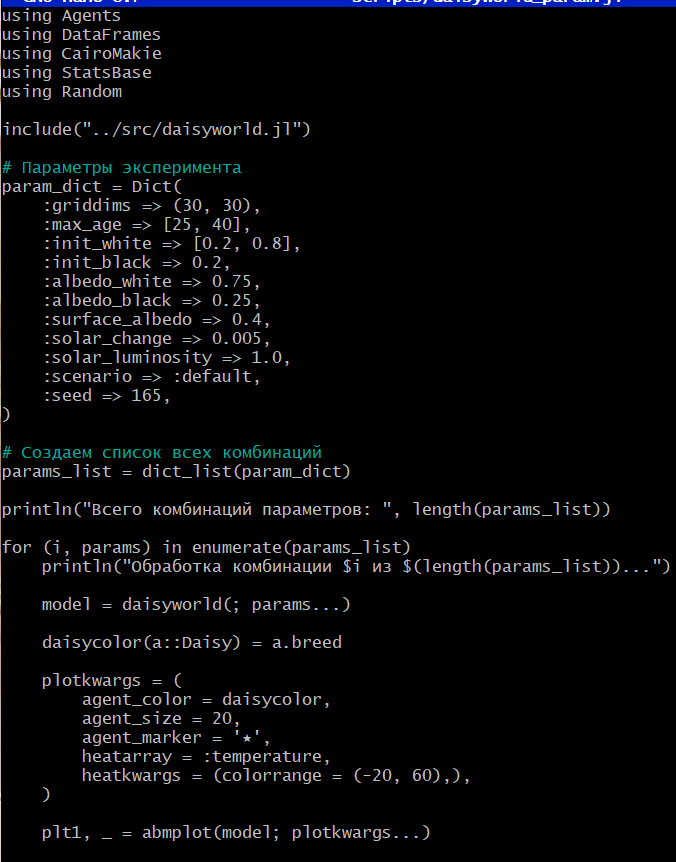
\includegraphics[keepaspectratio]{image/31.png}}

}

\caption{код}

\end{figure}%
\end{frame}

\begin{frame}{}
\phantomsection\label{section-22}
Запустила код

\begin{figure}[H]

{\centering \pandocbounded{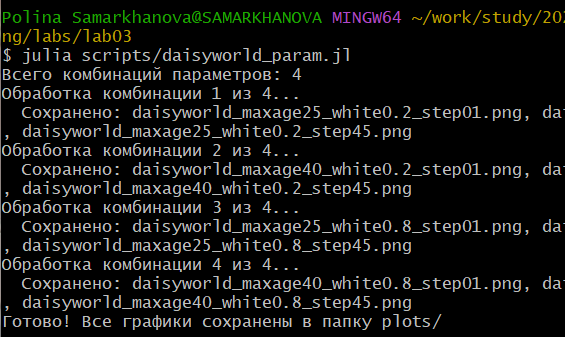
\includegraphics[keepaspectratio]{image/32.png}}

}

\caption{запуск}

\end{figure}%
\end{frame}

\begin{frame}{}
\phantomsection\label{section-23}
Посмотрела результат

\begin{figure}[H]

{\centering \pandocbounded{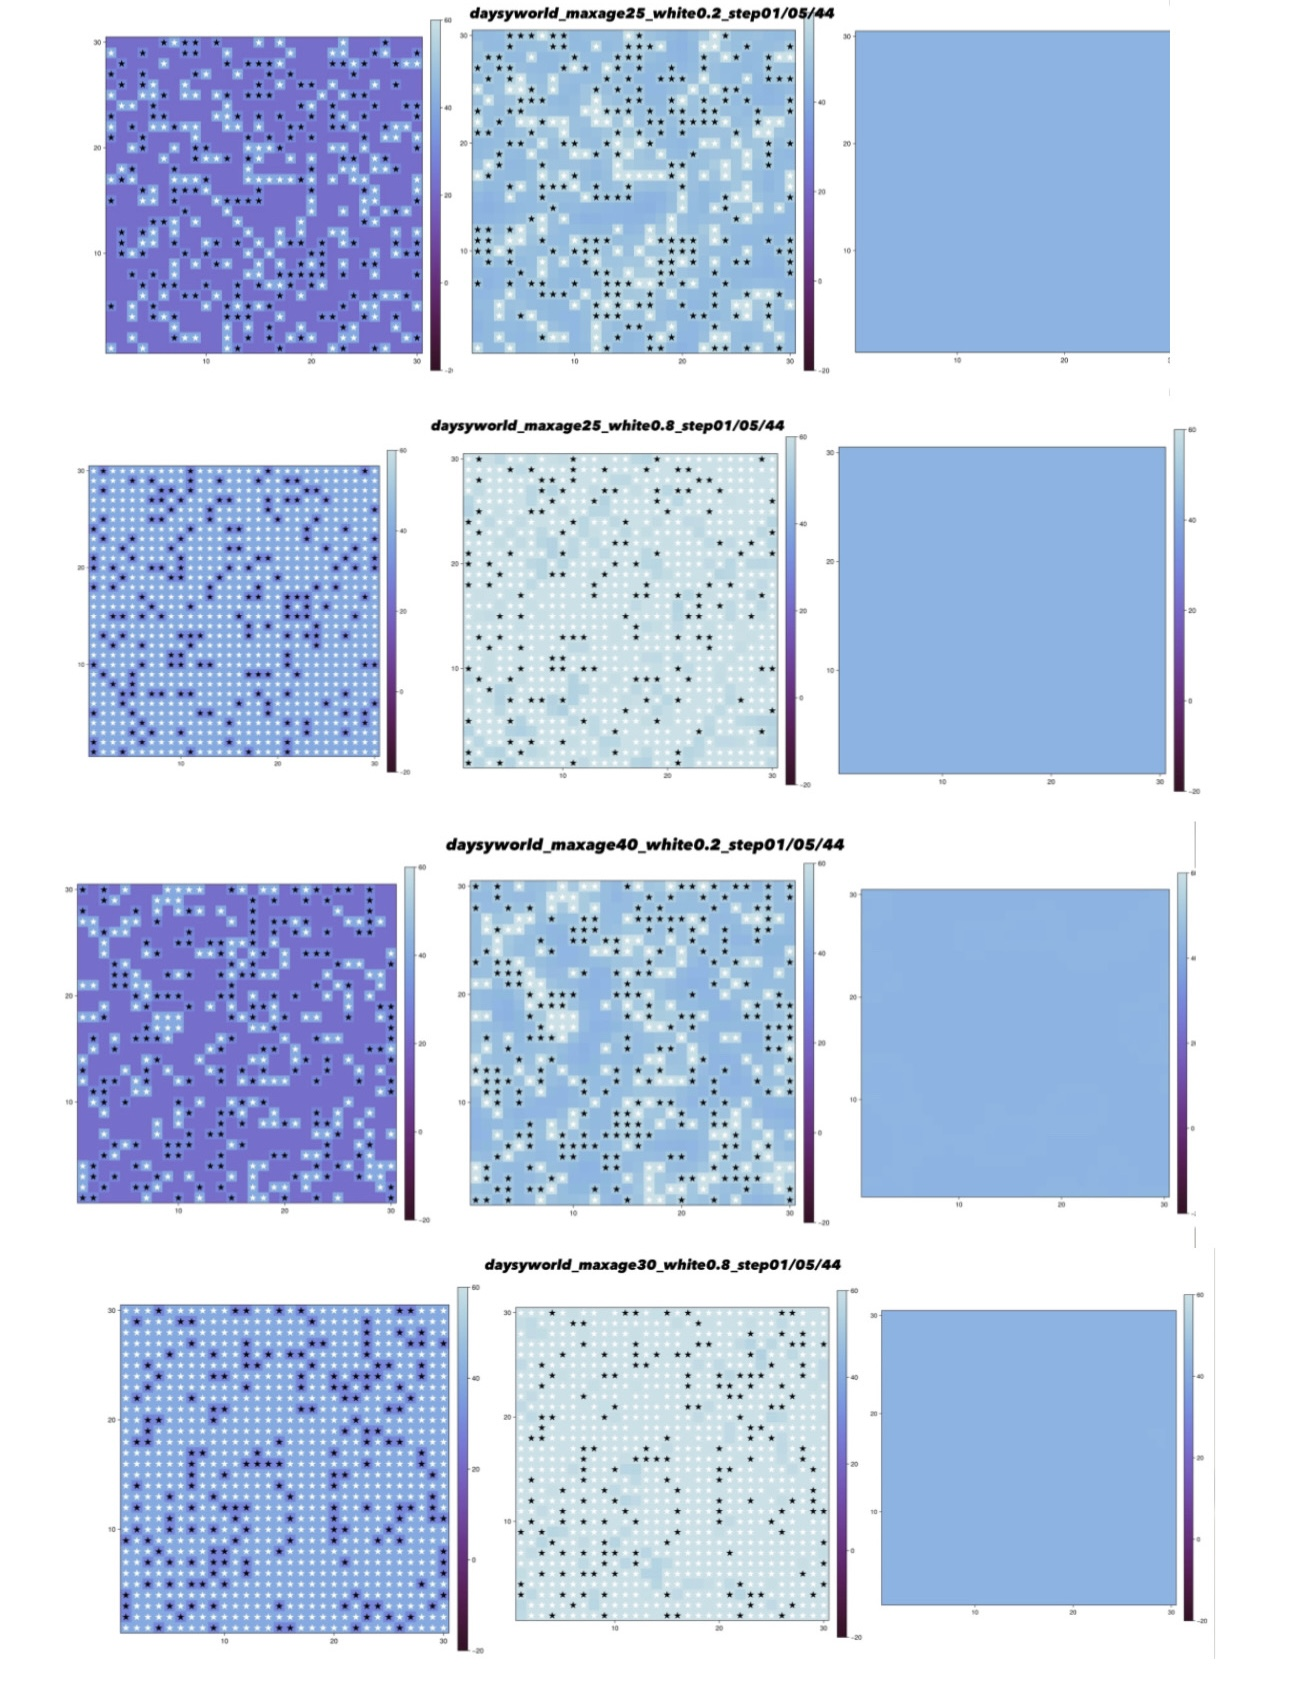
\includegraphics[keepaspectratio]{image/33.png}}

}

\caption{графики}

\end{figure}%
\end{frame}

\begin{frame}{Динамика числа маргариток(параметры)}
\phantomsection\label{ux434ux438ux43dux430ux43cux438ux43aux430-ux447ux438ux441ux43bux430-ux43cux430ux440ux433ux430ux440ux438ux442ux43eux43aux43fux430ux440ux430ux43cux435ux442ux440ux44b}
Создала файл scripts/daisyworld-count\_param.jl

\begin{figure}[H]

{\centering \pandocbounded{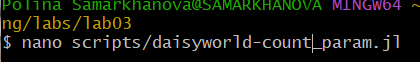
\includegraphics[keepaspectratio]{image/34.png}}

}

\caption{файл}

\end{figure}%
\end{frame}

\begin{frame}{}
\phantomsection\label{section-24}
В открывшемся окне вставила код из медодички

\begin{figure}[H]

{\centering \pandocbounded{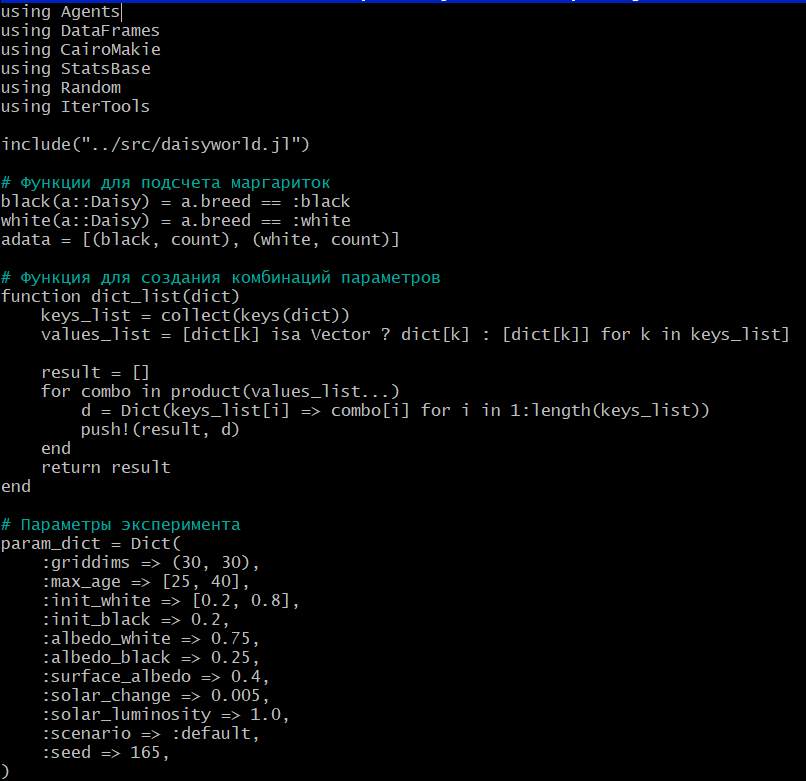
\includegraphics[keepaspectratio]{image/35.png}}

}

\caption{код}

\end{figure}%
\end{frame}

\begin{frame}{}
\phantomsection\label{section-25}
Запустила код

\begin{figure}[H]

{\centering \pandocbounded{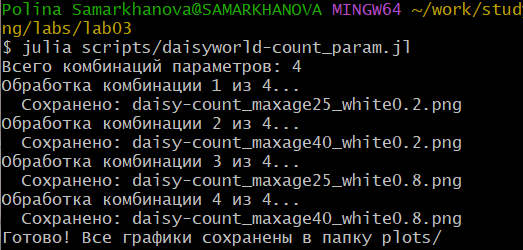
\includegraphics[keepaspectratio]{image/36.png}}

}

\caption{запуск}

\end{figure}%
\end{frame}

\begin{frame}{}
\phantomsection\label{section-26}
Посмотрела результат

\begin{figure}[H]

{\centering \pandocbounded{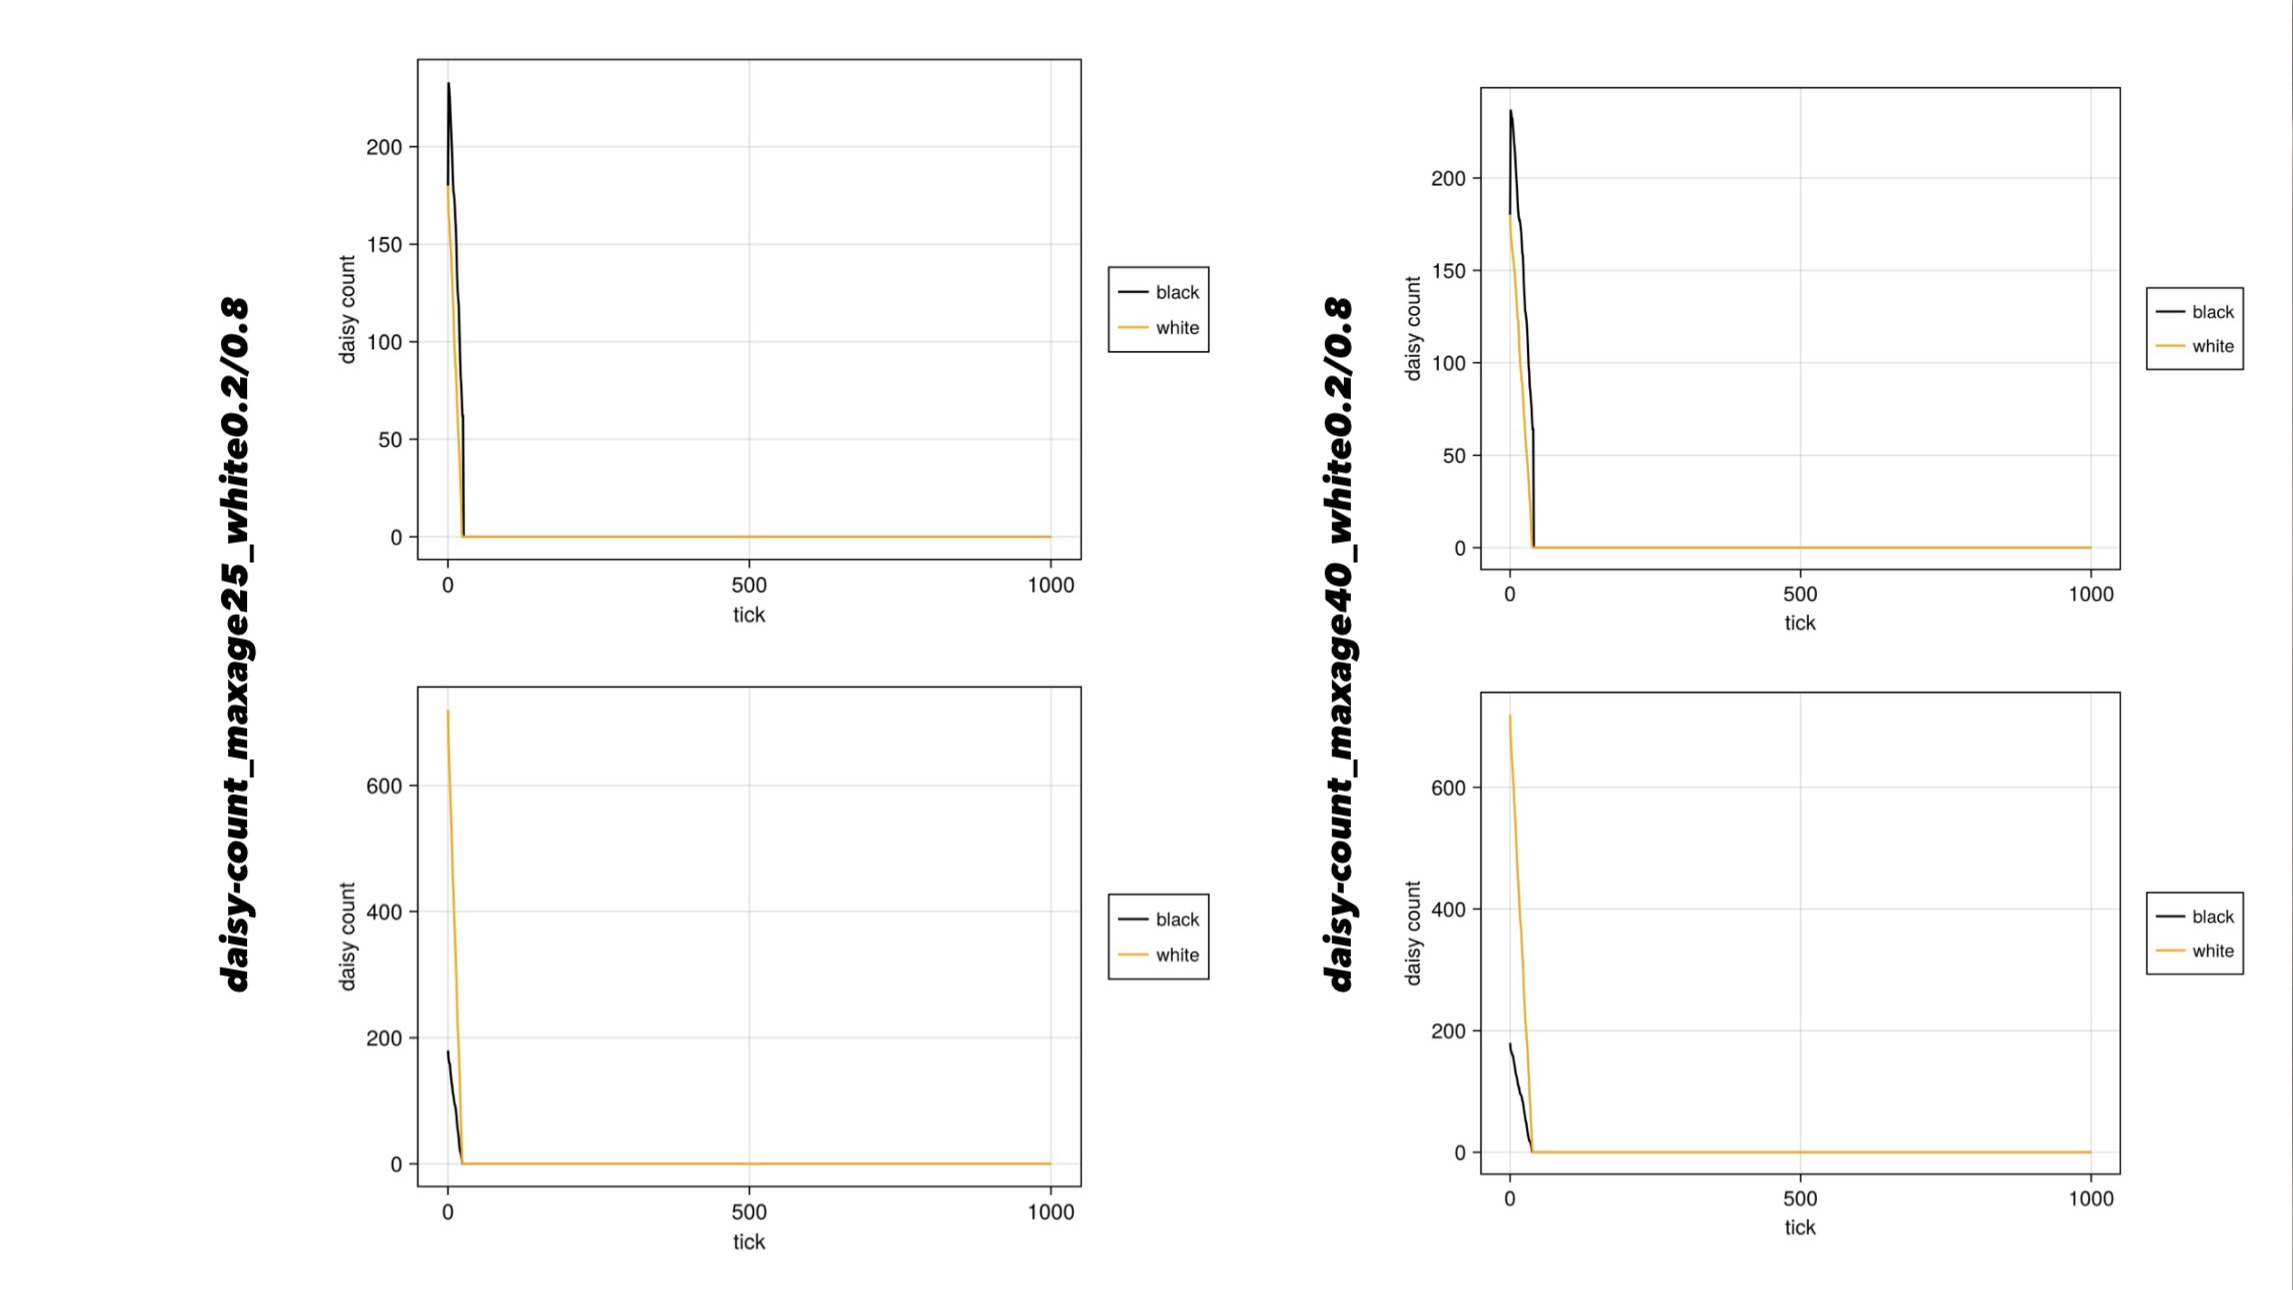
\includegraphics[keepaspectratio]{image/37.png}}

}

\caption{графики}

\end{figure}%
\end{frame}

\begin{frame}{Динамика модели(параметры)}
\phantomsection\label{ux434ux438ux43dux430ux43cux438ux43aux430-ux43cux43eux434ux435ux43bux438ux43fux430ux440ux430ux43cux435ux442ux440ux44b}
Создала файл scripts/daisyworld-luminosity\_param.jl

\begin{figure}[H]

{\centering \pandocbounded{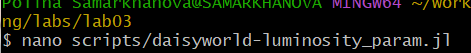
\includegraphics[keepaspectratio]{image/38.png}}

}

\caption{файл}

\end{figure}%
\end{frame}

\begin{frame}{}
\phantomsection\label{section-27}
В открывшемся окне вставила код из медодички

\begin{figure}[H]

{\centering \pandocbounded{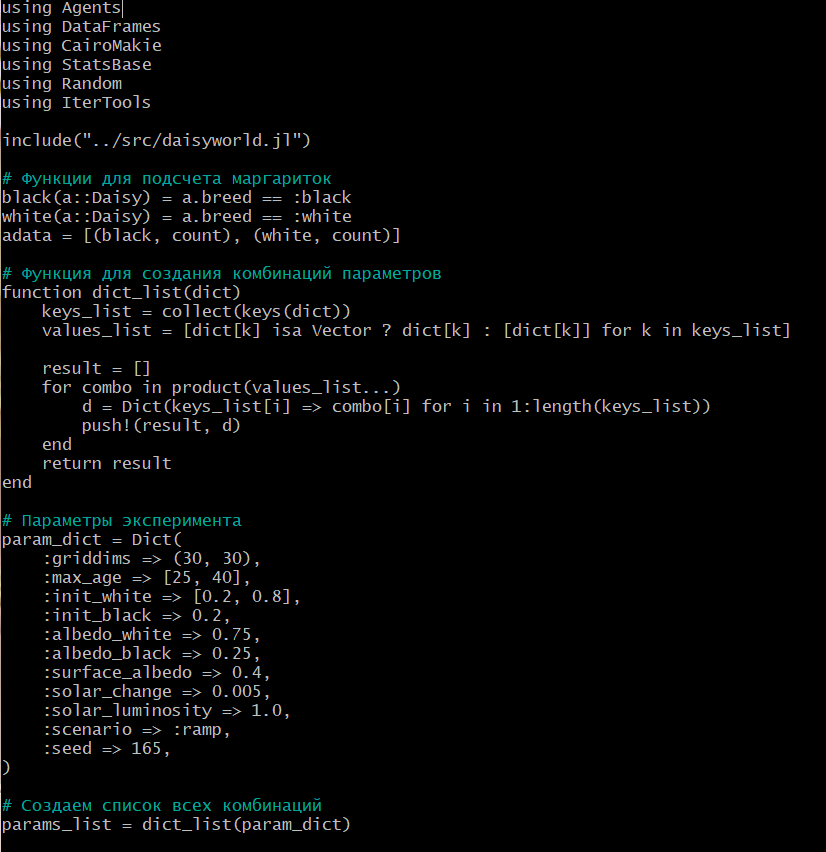
\includegraphics[keepaspectratio]{image/39.png}}

}

\caption{код}

\end{figure}%
\end{frame}

\begin{frame}{}
\phantomsection\label{section-28}
Запустила код

\begin{figure}[H]

{\centering \pandocbounded{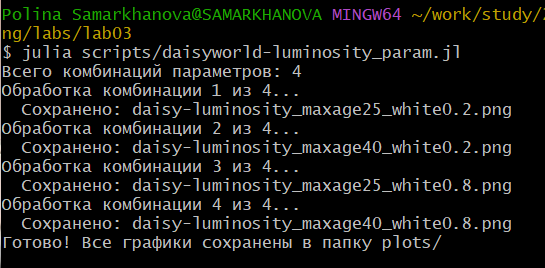
\includegraphics[keepaspectratio]{image/40.png}}

}

\caption{запуск}

\end{figure}%
\end{frame}

\begin{frame}{}
\phantomsection\label{section-29}
Посмотрела результат

\begin{figure}[H]

{\centering \pandocbounded{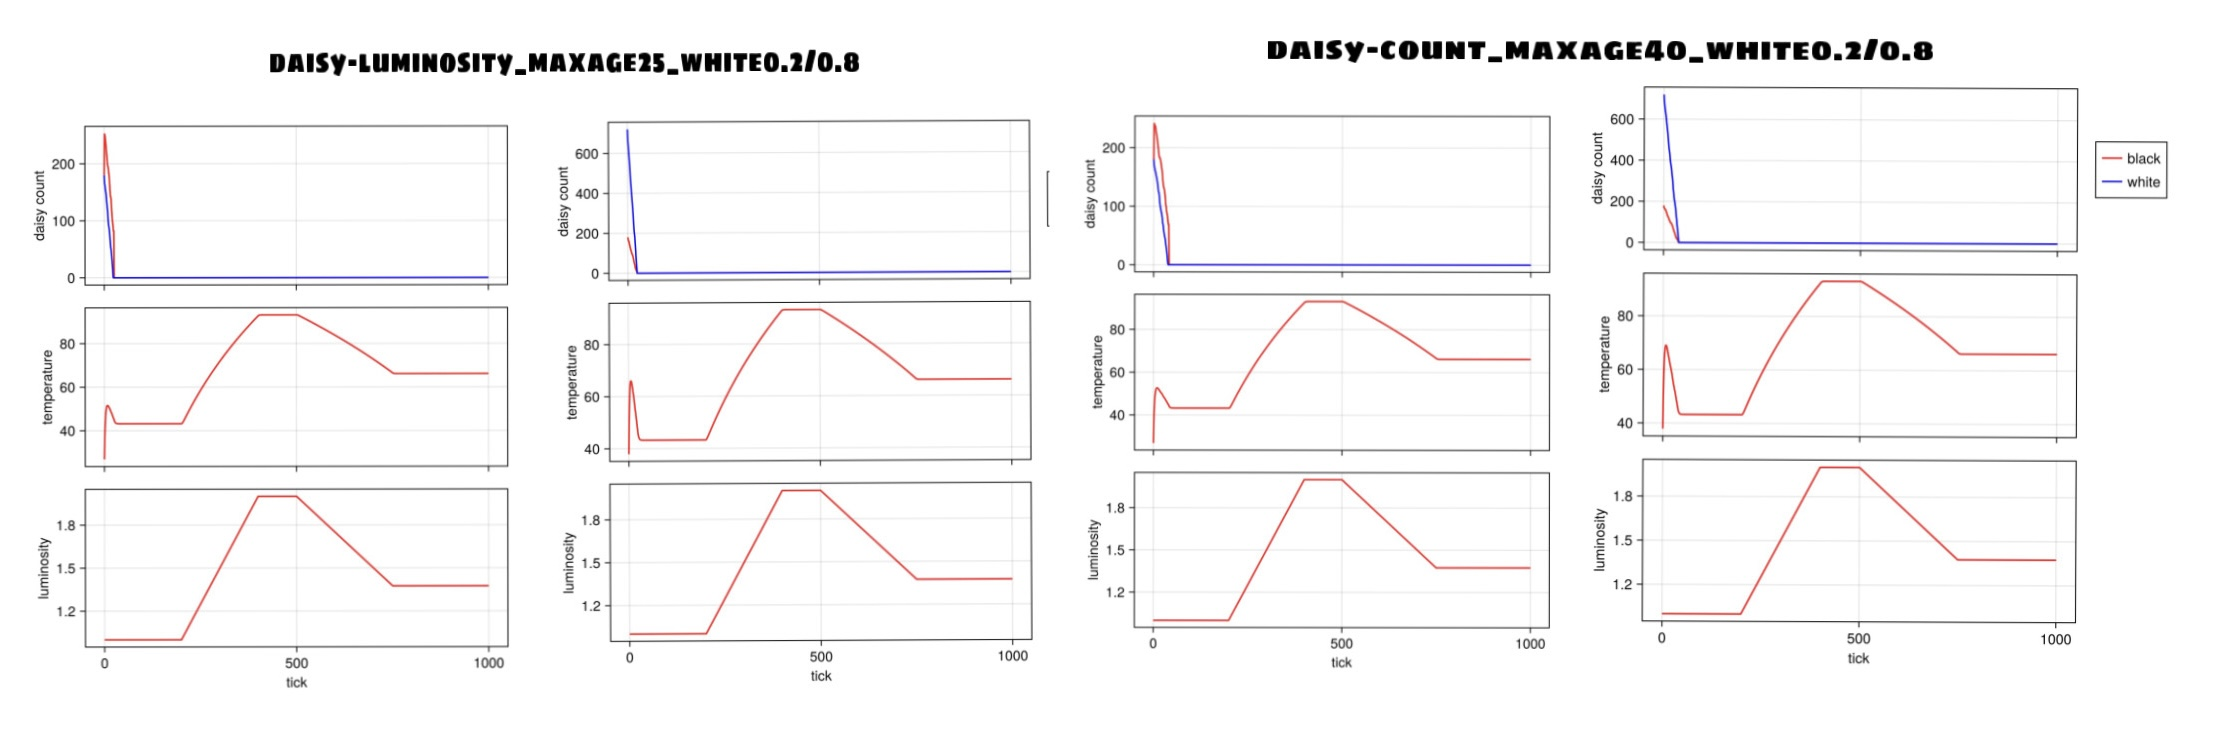
\includegraphics[keepaspectratio]{image/41.png}}

}

\caption{графики}

\end{figure}%
\end{frame}

\begin{frame}{}
\phantomsection\label{section-30}
Спасибо за внимание !
\end{frame}




\end{document}
